\chapter{Chirality}\label{sec:background:Chirality}
\section{Introduction}

\section{Chiroptical Effects}\label{sec:background:Chirality:Chiroptics}
\begin{figure}[htb!]
    \centering
    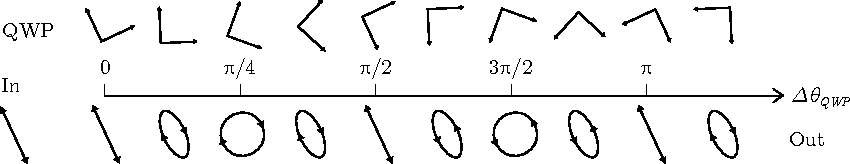
\includegraphics[scale=1.0]{./figures/background/chiroptics/QWP_in_out.pdf}
    \caption{\label{fig:QWP_in_out}Output polarisation from a QWP at an angle $\Delta\theta_{QWP}$ to the input polarisation. The angle of the input (and subsequent elliptical and linear outputs) is controlled by the half-wave plate.}
   \end{figure}

\subsection{Chiroptical Effects from Extrinsic Chirality}
\subsection{Chiroptical Effects from Anisotropy}

\section{Chirality Parameters}\label{sec:background:Chirality:Paremeters}
\begin{itemize}
    \item Introdution to chirality parameters in context of the field
\end{itemize}

\subsection{Structural Chirality}\label{sec:background:Chirality:Structural}
In the simple case of a linear, isotropic medium with no magnetoelectric coupling, the macroscopic electromagnetic response of the material is described by the constitutive relations given in equation~\ref{eq:background:chirality:isotropicConstitutive}. These relate the material’s internal electric displacement field $\bf{\tilde D}$ and magnetic field strength $\bf{\tilde D}$ to the driving electric and magnetic fields $\bf{\tilde E}$ and $\bf{\tilde B}$. Here, $\varepsilon$ and $\mu$ are complex (denoted by a tilde) scalars and correspond to the isotropic electric permittivity and magnetic permeability of the material.
\begin{equation}\label{eq:background:chirality:isotropicConstitutive}
	\begin{split}
        & \bf{\tilde D} = \tilde \varepsilon \bf{\tilde E} \\
        & \bf{\tilde B} = \tilde \mu \bf{\tilde H}
	\end{split}
\end{equation}
In the general case however, we cannot assume isotropy and a lack of magnetoelectric coupling. For a bi-anisotropic medium, the constitutive relations take the form of equation~\ref{eq:background:chirality:fullConstitutive}.\cite{Ishimaru2003, Capolino2009}. Here, $\bf{\tilde \varepsilon}$, $\bf{\tilde \mu}$, $\bf{\tilde \xi}$, and $\bf{\tilde \zeta}$ are $3 \times 3$ matrices due to the anisotropy of the material. $\bf{\tilde \xi}$, and $\bf{\tilde \zeta}$ describe the magneto-electric cross-coupling.
\begin{equation}\label{eq:background:chirality:fullConstitutive}
    \begin{bmatrix}
        \bf{\tilde D} \\
        \bf{\tilde B}
    \end{bmatrix}
    =
    \begin{bmatrix}
        \bf{\tilde \varepsilon} & \bf{\tilde \xi} \\
        \bf{\tilde \zeta} & \bf{\tilde \mu}
    \end{bmatrix}
    \begin{bmatrix}
        \bf{\tilde E} \\
        \bf{\tilde H}
    \end{bmatrix}
\end{equation}
In the case of a non-gyrotropic material (exhibiting no magneto-optic rotation), equation~\ref{eq:background:chirality:fullConstitutive} has additional constraints, due to time-reversal symmetry, given in equation~\ref{eq:background:chirality:nongyroConstraints} \cite{Ishimaru2003}.
\begin{equation}\label{eq:background:chirality:nongyroConstraints}
    \begin{split}
        &[\bf{\tilde \xi}]^t = -[\bf{\tilde \zeta}] \\
        &[\bf{\tilde \varepsilon}]^t = [\bf{\tilde \varepsilon}] \\
        &[\bf{\tilde \mu}]^t = [\bf{\tilde \mu}]
    \end{split}
\end{equation}
The expressions shown in equation~\ref{eq:background:chirality:isotropicConstitutive} are a special case of equation~\ref{eq:background:chirality:fullConstitutive}, where no magneto-electric cross-coupling is present, so $\bf{\tilde \xi}=\bf{\tilde \zeta}=0$ and due to isotropy, $\bf{\tilde \varepsilon}$ and $\bf{\tilde \mu}$ become scalars. 
In the case of a non-chiral anisotropic material, $\bf{\tilde \xi}=\bf{\tilde \zeta}=0$ however $\bf{\tilde \varepsilon}$ and $\bf{\tilde \mu}$ remain as matrices. Most relevant in this discussion however is the special case of a bi-isotropic, or isotropic chiral, medium. 
In this case the matrix components reduce to scalars, but all four components remain. The constraints given in equation~\ref{eq:background:chirality:nongyroConstraints} apply, and so we find that $\xi =-\zeta $.

There are several ways to write the remaining relations, including Post’s relations~\cite{Capolino2009}, Born’s relations~\cite{Lekner1999, Barnett2016} , and Tellegen’s relations~\cite{Capolino2009,kong1986,lindell1994} (equation~\ref{eq:background:chirality:tellegensRelations}). Tellegen’s relations will be used here, however the various forms are equivalent.
\begin{equation}\label{eq:background:chirality:tellegensRelations}
    \begin{bmatrix}
        \mathbf{D} \\
        \mathbf{B}
    \end{bmatrix}
    =
    \begin{bmatrix}
        \varepsilon_0 \varepsilon_r & i \kappa \sqrt{\mu_0 \varepsilon_0} \\
        -i \kappa \sqrt{\mu_0 \varepsilon_0} & \mu_0 \mu_r
    \end{bmatrix}
    \begin{bmatrix}
        \mathbf{E} \\
        \mathbf{H}
    \end{bmatrix}
\end{equation}
Here, ${{\varepsilon }_{r}}$ and $\mu_r$ are the relative permittivity and permeability of the material respectively, and $\kappa$ is known as the ``chirality parameter''. Solving Maxwell’s equations for a monochromatic plane wave propagating in the $z$ direction through the medium described by equation~\ref{eq:background:chirality:tellegensRelations} results in two eigenwaves with wave numbers given by equation~\ref{eq:background:chirality:kpmKappa}~\cite{Wang2014a, Qiu2008}, where ${{k}_{0}}$ is the wave number in vacuum. In a chiral medium these eigenwaves of wave number ${{k}_{+}}$ and ${{k}_{-}}$ correspond to left and right circularly polarized light respectively.
\begin{equation}\label{eq:background:chirality:kpmKappa}
    {k_\pm } = {k_0}\left( {\sqrt {{\mu _r}{\varepsilon _r}}  \pm \kappa } \right)
\end{equation}
From this, the corresponding refractive indices are given by equation~\ref{eq:background:chirality:npmKappa}~\cite{Capolino2009, Qiu2008, Valev2013b}. 
\begin{equation}\label{eq:background:chirality:npmKappa}
    {n_ \pm } = \sqrt {{\mu _r}{\varepsilon _r}}  \pm \kappa
\end{equation}
Since the refractive index is complex, $\operatorname{Re}(\kappa)$ corresponds to differential phase velocity for LCP and RCP light, resulting in optical rotation. $\operatorname{Im}(\kappa)$ corresponds to differential extinction of LCP and RCP light, resulting in circular dichroism. Optical rotation and circular dichroism are thus intrinsically linked by the Kramers-Kronig transforms.


\subsection{Optical Chirality}
The interaction between a chiral molecule and a chiral electromagnetic field is expected to exhibit a dissymmetry, in that each “handedness” of a chiral field should interact differently with a chiral molecule or nanostructure. A field with a shorter chiral pitch in the local EM field will exhibit a stronger interaction dissymmetry than a less twisted field. It had long been thought that the maximum possible chiral dissymmetry is obtained for a perfectly circularly polarized monochromatic field, however in 2010 Tang and Cohen proposed a setup in which the dissymmetry exceeds that of CPL (referred to as ``superchiral light'') at the nodes of a chiral standing wave.~\cite{Tang2010}
The strength of the field chirality can be quantified by Lipkin's 00-zilch density~\cite{Lipkin1964} referred to by Tang and Cohen as the ``optical chirality'' $C$ as given in equation~\ref{eq:background:chirality:opticalchirality}.
\begin{equation} \label{eq:background:chirality:opticalchirality}
    \begin{split}
        C = &\frac{\varepsilon_0 }{2}{\bf{\tilde E}} \cdot (\nabla  \times {\bf{\tilde E}}) + \frac{1}{{2\mu _0}}{\bf{\tilde B}} \cdot (\nabla  \times {\bf{\tilde B}}) \\
        = &- \frac{{{\varepsilon _0}\omega }}{2} \operatorname{Im}[ \bf{\tilde E}(\bf{r}) \cdot \bf{\tilde B}(\bf{r}) ]
    \end{split}
\end{equation}
Here, $\bf{\tilde E}$ and $\bf{\tilde B}$ denote the complex electric and magnetic field amplitudes respectively. This quantity describes the angular momentum of the curl of the optical field~\cite{Cameron2012a} and is a conserved property of the field. Tang and Cohen showed that the enantioselectivity of optical excitation of a molecule is highly dependent on $C$, and so it stands that such a superchiral field can lead to significant enhancement of the enantioselective excitation of chiral molecules.

The general response of a chiral molecule to a monochromatic electromagnetic field is described by an internal electric dipole moment $\mathbf{\tilde p}$ and magnetic dipole moment $\mathbf{\tilde m}$ as in equation~\ref{eq:background:chirality:tangDipole}.
\begin{equation}
    \label{eq:background:chirality:tangDipole}
    \begin{split}
        &{\bf{\tilde p}} = {{\tilde \alpha }_{ee}}{\bf{\tilde E}} - i{{\tilde \alpha }_{em}}{\bf{\tilde B}} \\
        &{\bf{\tilde m}} = i{{\tilde \alpha }_{em}}{\bf{\tilde E}} + {{\tilde \alpha }_{mm}}{\bf{\tilde B}}
    \end{split}
\end{equation}
Here, $\tilde{\alpha}_{ee}$ and $\tilde{\alpha}_{mm}$ correspond to $\tilde{\alpha}$ and $\tilde{\chi}$ in references~\cite{Tang2010} and~\cite{Choi2012}, 
$\alpha_{ee}$ is the electric polarizability, and $\alpha_{mm}$ is the magnetic susceptibility. $\tilde{\alpha}_{em}$ is the mixed magneto-electric polarizability and is directly related to the material chirality paremeter $\kappa$ (section~\ref{sec:background:Chirality:Structural}).
Physical quantities are obtained from the real parts of equation (14). For an incident $\mathbf{\tilde{E}}=\mathbf{\tilde{E}}_{0}{e}^{-i\omega t}$ and $\mathbf{\tilde{B}}=\mathbf{\tilde{B}}_{0}{e}^{-i\omega t}$ the rate of excitation of a molecule from right (+) and left (-) CPL is given by equation~\ref{eq:background:chirality:Aplusminus} \cite{Tang2010, Choi2012}.

\begin{equation} \label{eq:background:chirality:Aplusminus}
    {A^ \pm } = 
    \frac{\omega }{2}{\left\langle {{\bf{E}} \cdot {\bf{\dot p}} + {\bf{B}} \cdot {\bf{\dot m}}} \right\rangle _t} = 
    \frac{\omega }{2}{\mathop{\rm Im}\nolimits} ({{\bf{\tilde E}}^ * } \cdot {\bf{\tilde p}} + {{\bf{\tilde B}}^ * } \cdot {\bf{\tilde m}})
\end{equation}
Substituting equation~\ref{eq:background:chirality:tangDipole} into equation~\ref{eq:background:chirality:Aplusminus} leads to equation~\ref{eq:background:chirality:AplusminusFull}, which can be rewritten in terms of the generalized optical chirality $C$ to give equation~\ref{eq:background:chirality:AplusminusC}~\cite{Choi2012}. Here ${\tilde \alpha }_{em}''=\operatorname{Im}({\tilde \alpha }_{em})$.
\begin{equation} \label{eq:background:chirality:AplusminusFull}
    {A^ \pm } = \frac{\omega }{2}({\tilde \alpha ''_{ee}}{\left| {{\bf{\tilde E}}} \right|^2} + {\tilde \alpha ''_{mm}}{\left| {{\bf{\tilde B}}} \right|^2}) \pm {\tilde \alpha }_{em}''\omega {\mathop{\rm Im}\nolimits} ({{\bf{\tilde E}}^ * } \cdot {\bf{\tilde B}})
\end{equation}
\begin{equation} \label{eq:background:chirality:AplusminusC}
    {A^ \pm } \simeq \frac{\omega }{2}({\tilde \alpha ''_{ee}}{\left| {{\bf{\tilde E}}} \right|^2} + {\tilde \alpha ''_{mm}}{\left| {{\bf{\tilde B}}} \right|^2}) \pm {\tilde \alpha }_{em}''\frac{2}{\varepsilon }C
\end{equation}
The time averaged electric and magnetic energy densities ${{\left\langle {{U}_{E}} \right\rangle }_{t}}=\tfrac{\varepsilon }{4}{{\left| {\mathbf{\tilde{E}}} \right|}^{2}}$ and ${{\left\langle {{U}_{B}} \right\rangle }_{t}}=\tfrac{1}{4\mu }{{\left| {\mathbf{\tilde{B}}} \right|}^{2}}$  can be introduced here, and substituted into equation~\ref{eq:background:chirality:AplusminusC} to give the rate of excitation in terms of energy density as in equation~\ref{eq:background:chirality:AplusminusU}. 
\begin{equation}\label{eq:background:chirality:AplusminusU}
    \begin{split}
        & {A^ \pm } \simeq \frac{2}{\varepsilon }{{\tilde \alpha ''}_{ee}}\omega \left( {{{\left\langle {{U_E}} \right\rangle }_t} + \gamma {{\left\langle {{U_B}} \right\rangle }_t}} \right) \pm {\tilde \alpha }_{em}''\frac{2}{\varepsilon }C \\
        & \gamma  = \frac{{{{\tilde \alpha ''}_{mm}}}}{{{{\tilde \alpha ''}_{ee}}}}\varepsilon \mu  = \frac{{{{\tilde \alpha ''}_{mm}}}}{{{{\tilde \alpha ''}_{ee}}}}\frac{{{n^2}}}{{{c^2}}}
    \end{split}
\end{equation}
We can now define the dissymmetry factor $g$ of the chiroptical interaction by equation~\ref{eq:background:chirality:dissymmetryA}.
\begin{equation}\label{eq:background:chirality:dissymmetryA}
    g = \frac{{{A^ + } - {A^ - }}}{\frac{1}{2}({A^ + } + {A^ - })}
\end{equation}
In Tang and Cohen's proposal~\cite{Tang2010} the magnetic field was disregarded as negligible. Under this assumption, the dissymmetry factor is found to be 
\begin{equation}\label{eq:background:chirality:dissymmetryG}
    g =  - \frac{{{\tilde \alpha }_{em}''}}{{\tilde \alpha ''}_{ee}}\frac{{2C}}{{\omega {{\left\langle {{U_E}} \right\rangle }_t}}}
\end{equation}
Note that under this approximation, the dissymmetry factor splits into properties of the molecule only (${{\tilde \alpha }_{em}''}/{{\alpha }''}_{ee}$) and properties of the field only (${2C}/{\omega {{\left\langle {{U}_{E}} \right\rangle }_{t}}}$), however in the general case the dissymmetry factor cannot be separated in this way and is significantly more complex~\cite{Choi2012}.
The full expression accounting for magnetic energy density can be simplified by assuming a small dissymmetry factor such that $n_{LCP} \approx n_{RCP}$, to give equation~\ref{eq:background:chirality:dissymmetryFull}.~\cite{Choi2012}
\begin{equation}\label{eq:background:chirality:dissymmetryFull}
    g =  - \frac{{\tilde \alpha ''}_{em}}{{{\tilde \alpha ''}_{ee}}}\frac{{2C}}{{\omega [{{\left\langle {{U_E}} \right\rangle }_t} + \gamma {{\left\langle {{U_B}} \right\rangle }_t}]}}
\end{equation}
The limitation in chiroptical enhancement is now clear: at regions of low electric energy density, the magnetic energy density is maximized and should not be considered negligible. The $\gamma$ term in equation~\ref{eq:background:chirality:dissymmetryFull} is then the key limiting factor for the dissymmetry enhancement. The energy density terms in the denominator can no longer be reduced to arbitrarily small values in order to continually increase chiral dissymmetry. However, the chiral dissymmetry can still be increased by reducing the total electromagnetic energy density, increasing the structural chirality parameter of the medium, and increasing optical chirality $C$ of the electromagnetic field. 